\chapter{Trabalhos Relacionados}

\section{Introdução}

O presente capítulo apresenta os trabalhos relacionados à utilização de RNC para treinamento de imagens, com e sem variação de parâmetros; a trabalhos em que há a aplicação específica a versão 8 da YOLO; aqueles que utilizaram VANT e os que criaram automação para sistemas de Realidade Virtual. Objetiva-se com isso encontrar o estado da arte de cada trabalho, elencando as principais contribuições de cada trabalho.

No final do capítulo, compara-se os estudos de modo a justificar o presente sistema abordado neste trabalho. 

\section{Treinamento utilizando RNC e Alteração de Parâmetros da RNC}
\subsection{Identificação e Medição de Defeitos em Produtos Automotivos Usando Visão Computacional}

O trabalho apresentado por \cite{gonzaga2023identificaccao} investigou a aplicabilidade e eficácia de um sistema de visão computacional para identificar defeitos visuais, medindo os respectivos tamanhos, no controle de qualidade de uma empresa de reposição de vidros automotivos. A fim de automatizar a decisão de precificação dos itens defeituosos, de maneira replicável e confiável foi utilizada a RNC YOLOv5. 

Para o treinamento, foram analisadas 3.397 imagens com defeitos específicos da rotina da empresa. De todos esses, foram selecionadas 70% das fotos para treinamento e 30% das fotos para validação posterior ao treinamento. Cada defeito foi definido como uma classe marcada em cada foto. O processo de marcação \ref{fig:marcacao} da foto foi realizado no software labelImg \cite(labelimg). Foram marcadas nas fotos as seguintes classes: bolha, delaminação, manchas, irisação, ostra e grau, em vidros. Todas fotos foram utilizadas a partir de um dataset interno da empresa.

\begin{figure}[!h]
    \center
    \begin{minipage}{0.6\linewidth}
    \center
    \captionsetup{justification=centering,margin=0.5cm,font=small}
    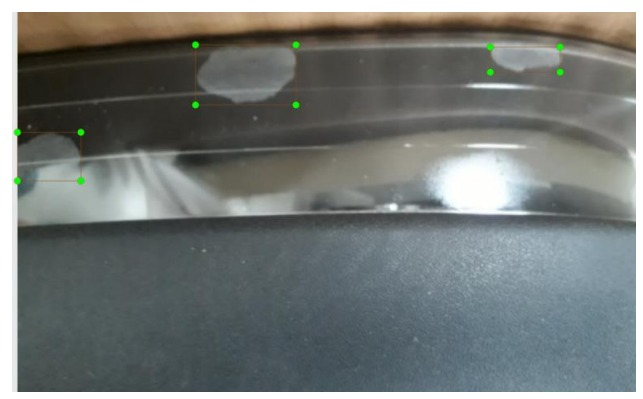
\includegraphics[width=0.7\linewidth]{img/cap3/mancha-marcacao.jpeg}
    \caption{ Exemplo de marcação de foto, utilizando labelImg, de um defeito em um vidro \cite{gonzaga2023identificaccao}} 
    \label{fig:mancha}
    \end{minipage}
\end{figure}

Para obtenção do melhor resultado, foram variados os tamanhos do valor do batch size (entre 2 e 32), além alterar para cada configuração desta, seu comportamento com três possibilidades de otimizadores diferentes: SGD, Adam e AdamW. A YOLO, em sua versão 5, oferece variações da arquitetura para diferentes propósitos. Neste trabalho, foram variadas 10 variações, juntamente com a alteração de parâmetros. Todos os outros hiperparâmetros foram mantidos na configuração padrão. Cada treinamento foi realizado em 300 épocas.

\begin{figure}[!h]
    \center
    \begin{minipage}{0.9\linewidth}
    \center
    \captionsetup{justification=centering,margin=0.5cm,font=small}
    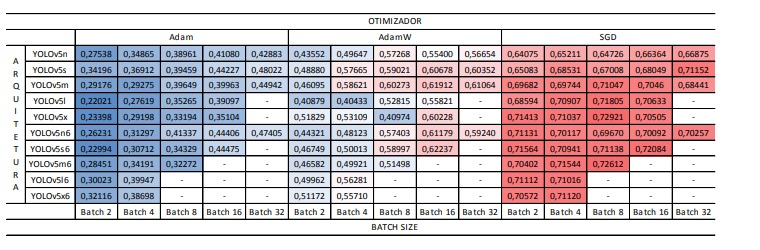
\includegraphics[width=0.7\linewidth]{img/cap3/tabela-mancha.jpeg}
    \caption{ Resultado do trabalho de \cite{gonzaga2023identificaccao}, variando os tipos de rede Yolo na versão 5, assim como o otimizador e o batch} 
    \label{fig:mancha}
    \end{minipage}
\end{figure}

O otimizador SGD, na variação YOLOv5x, com a o batch size de 8, alcançou a melhor precisão média, ou seja, um mAP de 0,72921. Com esta automatização, nos testes com a aplicação da detecção, houve uma precisão de 83,33% na precificação correta dos produtos defeituosos.

\section{Aplicação YOLOv8 e Utilização de VANT}
\subsection{Subseção 3}

\subsection{Subseção 4}

\section{Considerações Finais}

Inserir considerações finais. 


\begin{table}[!hbt]
\centering
\caption{Resumo comparativo dos trabalhos relacionados}
\begin{tabular}{ >{\centering\arraybackslash}m{5cm} | >{\centering\arraybackslash}m{1.5cm} | >{\centering\arraybackslash}m{2cm} | >{\centering\arraybackslash}m{2cm} | >{\centering\arraybackslash}m{1.5cm} | >{\centering\arraybackslash}m{1.5cm} | >{\centering\arraybackslash}m{2cm} }
\hline
\cellcolor[gray]{0.9} \textbf{Trabalhos Relacionados} & 
\cellcolor[gray]{0.9} \begin{sideways} \textbf{Treinamento utilizando RNC} \end{sideways} & 
\cellcolor[gray]{0.9} \begin{sideways} \textbf{Alteração de Parâmetros da RNC} \end{sideways} & 
\cellcolor[gray]{0.9} \begin{sideways} \textbf{Aplicação YOLOv8} \end{sideways} & 
\cellcolor[gray]{0.9} \begin{sideways} \textbf{Utilização de VANT} \end{sideways} & 
\cellcolor[gray]{0.9} \begin{sideways} \textbf{Subestações de Energia} \end{sideways} &
\cellcolor[gray]{0.9} \begin{sideways} \textbf{Automação de Inserção de RV} \end{sideways} \\
\hline 
\cite{gonzaga2023identificaccao} & \(\checkmark\) & \(\checkmark\) & \(\times\) & \(\times\) & \(\times\) & \(\times\) \\
\hline
\end{tabular}
\label{tab:relacionado1}
\end{table}
A tabela \ref{tab:relacionado1} apresenta um resumo de todos os trabalhos relacionados descritos nesse capítulo, considerando os seguintes temas:

\begin{itemize}
\item \textit{Treinamento utilizando RNC}: utilização de RNC para realizar treinamento em conjunto de imagens;
\item \textit{Alteração de Parâmetros da RNC para treinamento}: variação de parâmetros como batch e otimizadores para treinamento;
\item \textit{Automação de Inserção de RV}: construir sistema de inserção automática de objetos em um sistema de RV;
\item \textit{Aplicação YOLOv8}: utilização da versão 8 da YOLO para realizar treinamentos;
\item \textit{Utilização de VANT}: realizar coleta de fotos utilizando VANT; e
\item \textit{Subestações de Energia}: realizar toda coleta, treinamento e inserção voltado para Subestações de Energia. 
\end{itemize}
    
Pela análise da Tabela \ref{tab:relacionado1}, it is possible to note that until the present moment, a system with all features above, has not been found in the literature. It's believed that through these features, the user and therapist will be connected to a training environment and interacting in a more natural, secure, and efficient way. The idea is to have a user who, from any place with Internet and a computer, will issue commands necessary to control a PW and, at the same time, will receive visual augmented feedback in a traditional monitor device. Each user has different impairments and thus the therapist can set up a specific amount of tasks that will make part of the training protocol.  Therefore, this research proposes the investigation of computer techniques that support the integration of all these features.

No próximo capítulo, detalha-se os materiais e métodos uitlizados para a solução proposta.

